% !TeX program = pdflatex
\documentclass[tikz,border=8pt]{standalone}
\usepackage{pgfplots}
\pgfplotsset{compat=1.16}
\definecolor{FigureBlue}{HTML}{2563EB}
\definecolor{FigureOrange}{HTML}{EA580C}
\definecolor{FigureSlate}{HTML}{64748B}
\begin{document}
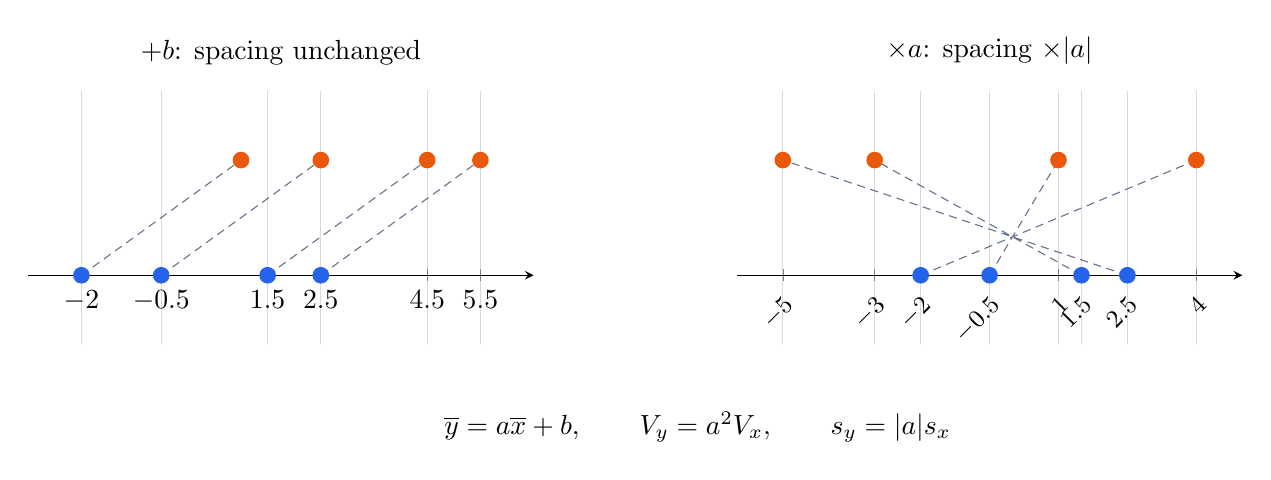
\begin{tikzpicture}
  \begin{axis}[
    width=8cm,height=4.8cm,xmin=-3,xmax=6.5,ymin=-.6,ymax=1.6,
    axis x line=middle,axis y line=none,ytick={0,1},yticklabels={$X$,$X+3$},
    xtick={-2,-.5,1.5,2.5,4.5,5.5},grid=both,clip=false,title={$+b$: spacing unchanged},
    grid style={draw=gray!18},major grid style={draw=gray!30},
  ]
    \addplot[only marks,mark=*,mark size=2.8pt,FigureBlue] coordinates {(-2,0) (-.5,0) (1.5,0) (2.5,0)};
    \addplot[only marks,mark=*,mark size=2.8pt,FigureOrange] coordinates {(1,1) (2.5,1) (4.5,1) (5.5,1)};
    \draw[FigureSlate,densely dashed] (axis cs:-2,0)--(axis cs:1,1) (axis cs:-.5,0)--(axis cs:2.5,1) (axis cs:1.5,0)--(axis cs:4.5,1) (axis cs:2.5,0)--(axis cs:5.5,1);
  \end{axis}
  \begin{axis}[
    at={(9cm,0)},anchor=south west,width=8cm,height=4.8cm,xmin=-6,xmax=5,ymin=-.6,ymax=1.6,
    axis x line=middle,axis y line=none,ytick={0,1},yticklabels={$X$,$-2X$},
    xtick={-5,-3,-2,-.5,1,1.5,2.5,4},grid=both,clip=false,title={$\times a$: spacing $\times|a|$},
    xticklabel style={font=\small,rotate=45,anchor=north east},
    grid style={draw=gray!18},major grid style={draw=gray!30},
  ]
    \addplot[only marks,mark=*,mark size=2.8pt,FigureBlue] coordinates {(-2,0) (-.5,0) (1.5,0) (2.5,0)};
    \addplot[only marks,mark=*,mark size=2.8pt,FigureOrange] coordinates {(4,1) (1,1) (-3,1) (-5,1)};
    \draw[FigureSlate,densely dashed] (axis cs:-2,0)--(axis cs:4,1) (axis cs:-.5,0)--(axis cs:1,1) (axis cs:1.5,0)--(axis cs:-3,1) (axis cs:2.5,0)--(axis cs:-5,1);
  \end{axis}
  \node at (8.5,-1.05) {$\overline{y}=a\overline{x}+b,\qquad V_y=a^2V_x,\qquad s_y=|a|s_x$};
\end{tikzpicture}
\end{document}
